\documentclass[10pt, conference]{lib/IEEEtran}

\usepackage{graphicx}
\usepackage{color}
\usepackage{epstopdf}
\usepackage{amsmath}
\usepackage{float}
\usepackage[font=small]{caption}

\begin{document}

\title{Performance Analysis of TCP Variants}

\author{\IEEEauthorblockN{Zhemin Mi}
\IEEEauthorblockA{College of Engineering\\
Northeastern University, MA, 02115\\
Email: mi.z@husky.neu.edu\\}
\and
\IEEEauthorblockN{Binbin Lu}
\IEEEauthorblockA{College of Engineering\\
Northeastern University, MA, 02115\\
Email: lu.b@husky.neu.edu\\}
}
\maketitle


\begin{abstract}
This paper simulated and analyzes the performance between different TCP variants on a simple network topology with a tool called NS-2. The key comparision factors this looking for between TCP variants are latency, drop rate, throughput and fairness. Multiple experiments were simulated against Tahoe, Reno, NewReno and Vegas. Finally, this paper investigated the queuing influences with TCP Reno and SACK.
\end{abstract}


\section{Introduction}
The original design of the Transmission Control Protocol (TCP) worked 
reliably, but was unable to provide acceptable performance in large 
and congested networks. Several TCP variants have been proposed since 
then (TCP Tahoe, Reno, NewReno, Vegas, BIC, CUBIC, SACK, and others) 
with mechanisms to control and avoid congestion. In this paper, we 
performed a couple of simulations using NS-2 to compare the 
performance of TCP Tahoe, Reno, NewReno and Vegas under same topology. 
In experiment1, we investigated the throughput, drop rate and latency 
under a certain congestion, which is simulated by a UPD based Constant 
Bit Rate (CBR); In experiment2, this paper compares the fairness 
between Reno/Reno, NewReno/Reno, Vegas/Vegas and NewReno/Vegas under 
simular variants congestion as experiment1; In experiment3, we learned 
the impact of queuing disciplines, DropTail and Random Early Drop (RED)
, on TCP Reno and SACK.


\section{Experiment 1: TCP Performance Under Congestion}
The network topology and flow setup of experiment 1 is as figure~\ref{fig:exp1_tpg}.
\begin{figure}[!htb]
    \centering
    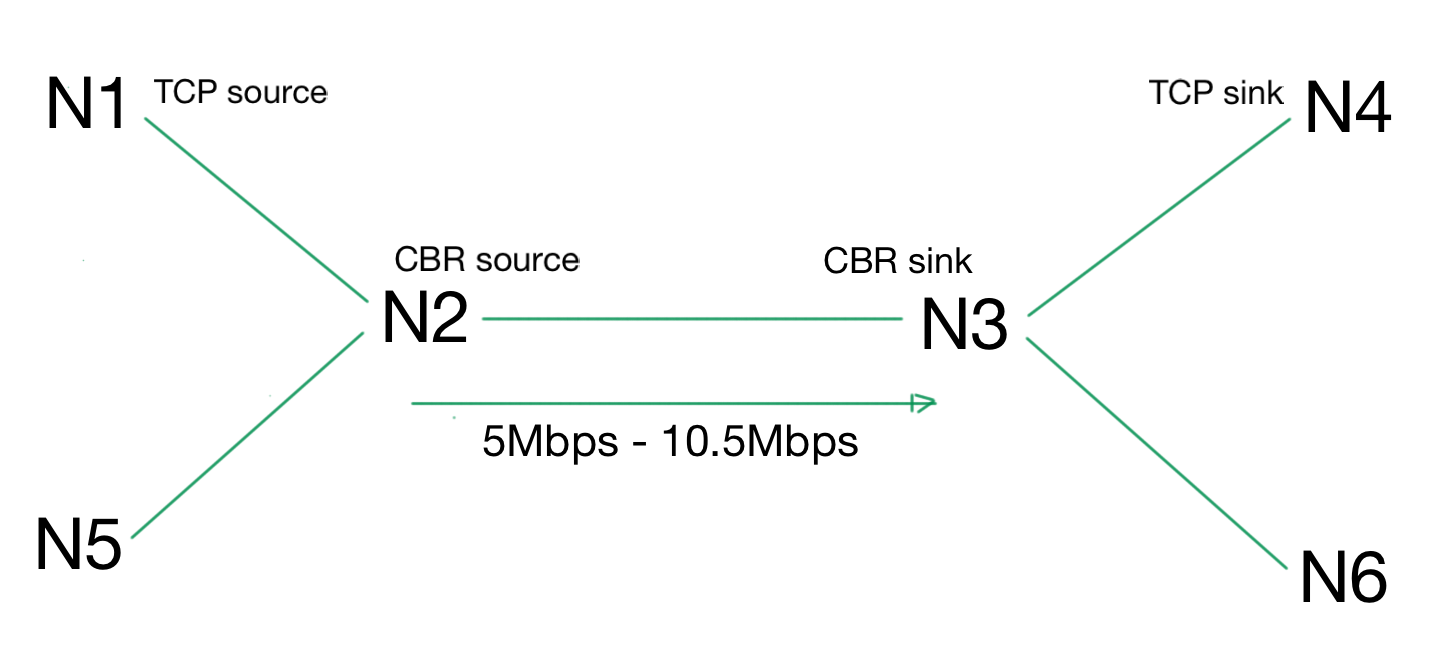
\includegraphics[width=0.8\linewidth]{images/top_exp1.png}
    \caption{Experiment 1 Network Topology}
    \label{fig:exp1_tpg}
\end{figure}
The methodology of this experiment is simple and straightforward: we 
build the topology first, then start the CBR flow from N2 to N3 and 
TCP flow from N1 to N4 later. In each separate simulation, the CBR rate
is steady and from the range of 5Mbps and 10.5Mbps, TCP flow is one of 
TCP Tahoe, Reno, NewReno and Vegas. The CBR rate increases 0.5Mbps 
every time and we run simulations for each TCP variant against all 
rates. For a single TCP variant and a single CBR rate, about 100 
simulations were performed by slightly veried start time of TCP flow. 
We did this to get the average and standard deviation of each result 
for later t-test, to make sure the difference were statistically 
different from each other, which means the protocol caused the 
difference rather than noise or randomness. 

Because CBR has no flow control algorithm, the increase of sending 
rate will gradually fill the pipe between N2 and N3, which will cause 
congestion in the TCP flow. Differenct TCP variants have different 
congestion control algorithms, but they all should slow down the 
sending rate to coordinate with the situation. Also, congestion will 
increase the latency and packet drop rate of TCP flow. We can verify each of them in experiment1.

\subsection{Throughput}
After running the NS-2 simulation tool. a detailed simulation results 
contain all events (CBR and TCP) will be generated. We calculated the
 throughput by filtering the ACK events in N1. Everytime we receive an
 un-duplicate ACK, we know a packet has been successfully delivered. 
 The simulation result is shown in figure~\ref{fig:exp1_thp}.
\begin{figure}[!htb]
    \centering
    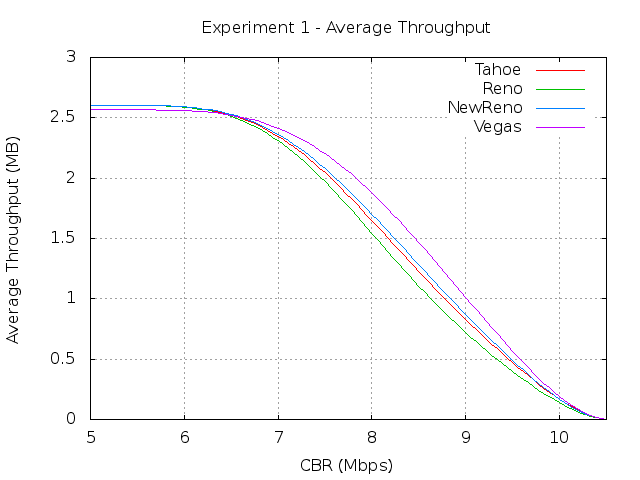
\includegraphics[width=1.0\linewidth]{plot/exp1-thp.png}
    \caption{Throughput of TCP variants}
    \label{fig:exp1_thp}
\end{figure}
For low CBR rate (e.g. CBR$ \le 6.5$Mbps), the througput of all four TCP 
variants are steady and about in the same value, with Vegas having a 
slightly lower throughput than the others. As CBR rate continues 
increase, all four TCP variants start to suffer the congestion. It is 
clearly shows that Vegas performs best in average througput, and Reno
performs the worst. The reason behind this is that Vegas is able to 
detect the congestion earlier than other variants by seeing the 
increasing Round Travel Time (RTT) values. In this way, Vegas is more 
likely to send more data while the others have to wait for timeouts or 
duplicate ACKs. But under a good network, Vegas is more senstive and 
conducts more congestion control, which makes it has lower throughput 
than others.

\subsection{Packets Drop Rate}
In the generated trace file by NS-2, drop packets at each node are 
labored with ``d'' sign. However, packets can be lost in either nodes 
or links, so we decide to calculate the lost packet by our own. We 
set a counter TOTAL-PACKET for sent packet at N1, and another counter 
EFFECTIVE-ACK for effecitve ACK (un-duplicate ACK). This way, the drop 
can be described in figure~\ref{fig:exp1_drop}.
\begin{figure}[!htb]
    \centering
    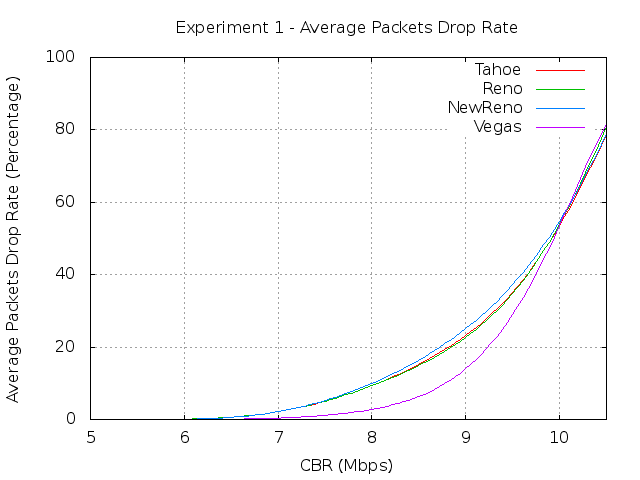
\includegraphics[width=1.0\linewidth]{plot/exp1-dr.png}
    \caption{Packets Drop Rate of TCP variants}
    \label{fig:exp1_drop}
\end{figure}
When CBR rate is below 6Mbps, no packet dropped for all four TCP 
variants. Clearly, Vegas performs better than the other three variants 
again, for two reasons. Firstly, TCP Tahoe, Reno and NewReno start to 
have dropped packets earlier than Vegas; and secondly, Vegas has 
relatively lower drop rate under all congestion conditions. Though 
Vegas has a little higher drop rate when CBR rate is bigger than 
10Mbps, it cannot deny the better ``most-conditions'' performance of 
Vegas.


\subsection{Latency}
There is no clear information in the trace file about latency, so we 
have to calculate it by our own based on the RTT. We used an array of 
floats $sentPacket$ to keep track of the sent time of each packet. 
Noticed that:
\begin{center}
    $T_{avg\_latency} = \dfrac{\sum_{i = 0}^{n - 1} (T_{ack}^i - T_{send}^i)}{sentPackets.size()}$
\end{center}
we only need another counter $totalTime$ to calculate the total transmitted time 
for later use.
Initially, all entries were set to $-1$. Everytime we detected a 
``enqueue'' at N1, we set the coressponding entry (same as packet seq 
number) to current time. Whenever we receive an valid ACK, the RTT for 
this packet was added to $totalTime$, and corresponding entry in 
$sentPackets$ is set back to -1. 
\begin{enumerate}
    \item For retransmitted packet, the sent time is the time when it firstly sent out.
    \item If we receive a ACK with corresponding entry value is -1, either it is a duplicate ACK, or an error. In both cases, we ignore the ACK.
\end{enumerate}
When the TCP flow stops, we can calculate the average latency with:
\begin{center}
    $T_{avg\_latency} = \dfrac{totalTime}{sentPackets.size()}$
\end{center}
The average latencies for the four TCP variants are showed in figure~\ref{fig:exp1_lt}
\begin{figure}[!htb]
    \centering
    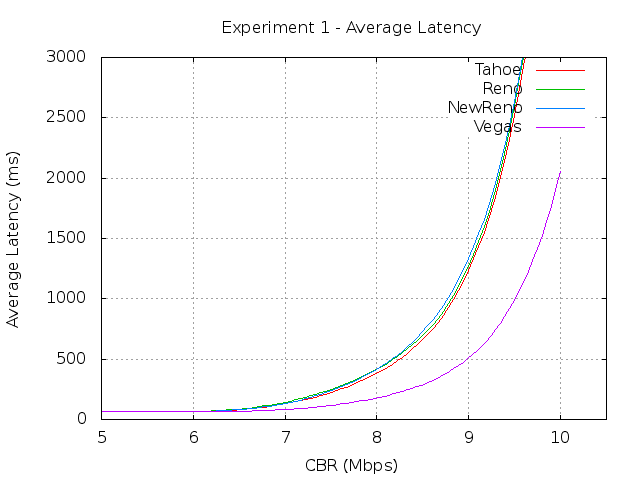
\includegraphics[width=1.0\linewidth]{plot/exp1-lt.png}
    \caption{Average Latency of TCP variants}
    \label{fig:exp1_lt}
\end{figure}
The results is similar to the other two: At a fairly low CBR rate 
(e.g. CBR rate$ \le 6$Mbps), all TCP variants performs well, the 
average latency is almost the same as optimal (60ms). As CBR rate 
continues increase, all TCP variants start to suffer longer delay, 
while Vegas has much lower latency than the other three. At 10Mbps 
CBR rate, Vegas is the only one still ``survives'', all other variants
are having too long latency, which means the packets are not likely 
delivered.

\subsection{T-Test}
The above three results show that there are differences in performance 
those four TCP variants. But we need to make sure it is caused by the
TCP protocols themselves, not by noise or randomness. Since we run the 
tests agains each variant at a certain CBR rate for 100 times, we can
perform the T-Test by using the mean and standard deviation. 
\begin{center}
    $t = \dfrac{\bar{x}_T -\bar{x}_C}{\sqrt{\frac{Var_T}{n_T} + \frac{Var_C}{n_C}}}$
\end{center}
The bigger the t is, the more likely that the difference between group T and group C are confidential. And figure~\ref{fig:exp1_t_test}
\begin{figure}[!htb]
    \centering
    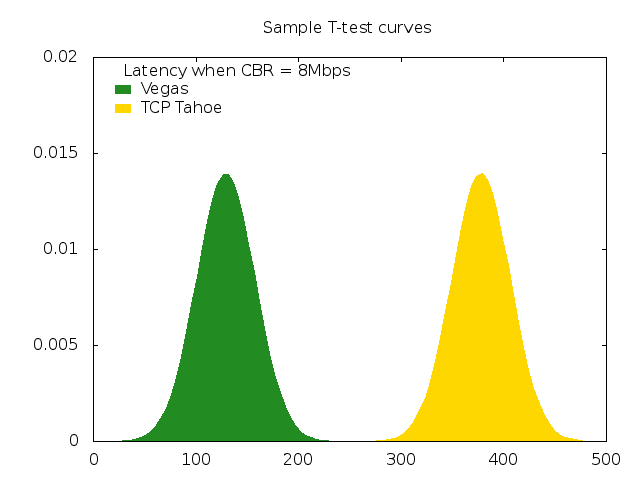
\includegraphics[width=1.0\linewidth]{plot/exp1-t-test.png}
    \caption{Sample T-test figure}
    \label{fig:exp1_t_test}
\end{figure}
is one of the t-test results. Other comparisions show similar results.
Clearly, it is due to the implementation of Vegas rather than noise 
that makes it better than other three variants.


In experiment1, we see that under a non-congested network, all four TCP
variants perform fairly the same, with low latency, good throughput and
zero drop rate. As the congestion increases, Vegas stands out in all 
three factors. However, we can still not confirm that Vegas is the best
TCP implementation of all four, because experiment 1 runs in a simple
topology. It requires a more complicated environment to confirm on that.




\section{Experiment 2: Fairness Between TCP Variants}
The network topology and flow setup of experiment 2 is as figure~\ref{fig:exp2_tpg}.
\begin{figure}[!htb]
    \centering
    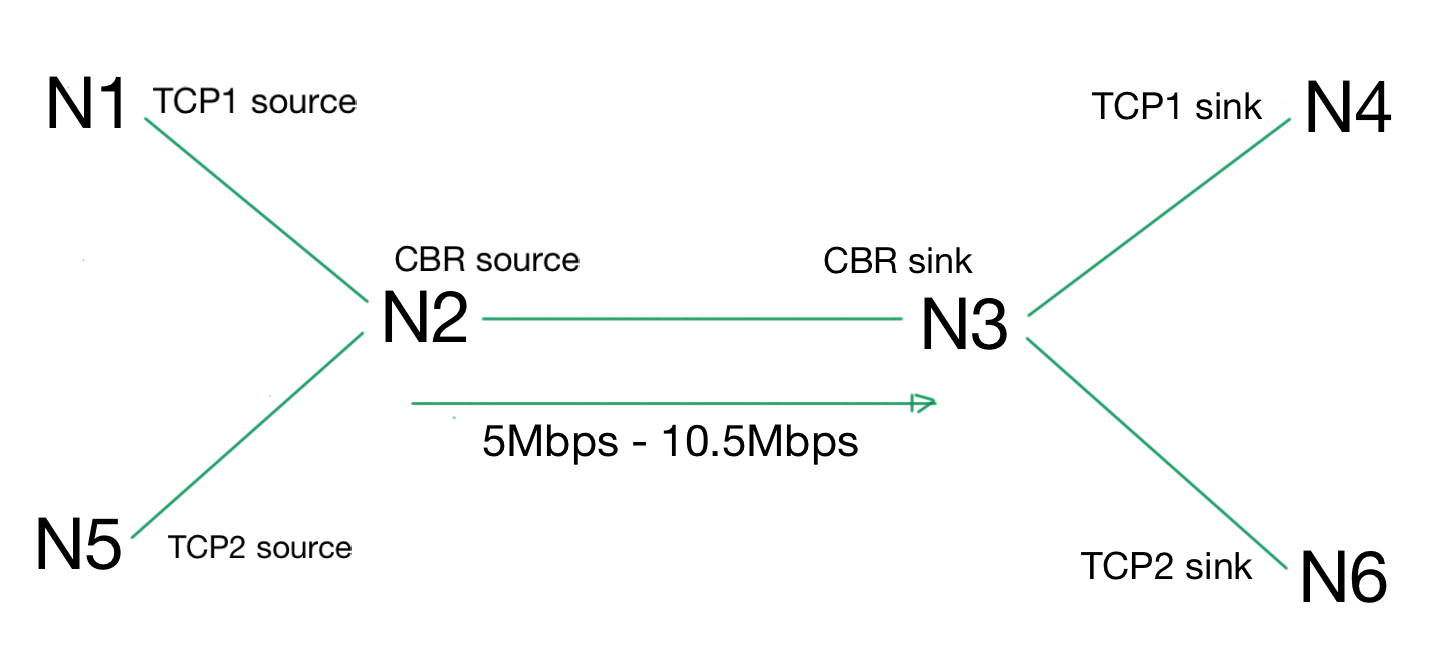
\includegraphics[width=0.8\linewidth]{images/top_exp2.png}
    \caption{Experiment 2 Network Topology}
    \label{fig:exp2_tpg}
\end{figure}
In experiment2, we still evaluate the TCP performance with the three 
same factors as those in experiment1: Throughput, Packet Drop Rate and 
Transmission Latency. Instead of having only one TCP flow in the 
topology, this time we are having two, running same or different TCP 
variants. We want to learn the fairness of each TCP variant.


\subsection{Reno/Reno and Vegas/Vegas}
For this simulation, we want to compare the fairness between Reno/Reno and Vegas/Vegas,
to see if these protocols are fair to themselves. Figure ~\ref{fig:exp2_thp_rr}, figure~\ref{fig:exp2_dr_rr} and figure~\ref{fig:exp2_dr_rr} shows the Throughput, Packet Drop Rate and Latency, respectively.
\begin{figure}[H]
    \centering
    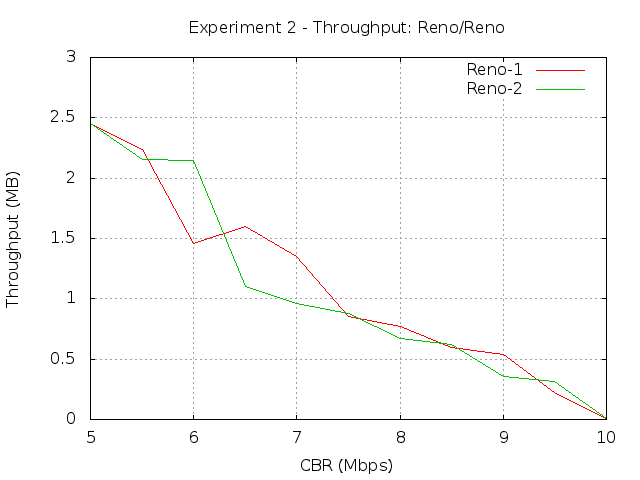
\includegraphics[width=1.0\linewidth]{plot/exp2-thp-Reno-Reno.png}
    \caption{Fairness of Throughput on Reno/Reno}
    \label{fig:exp2_thp_rr}
\end{figure}
\begin{figure}[H]
    \centering
    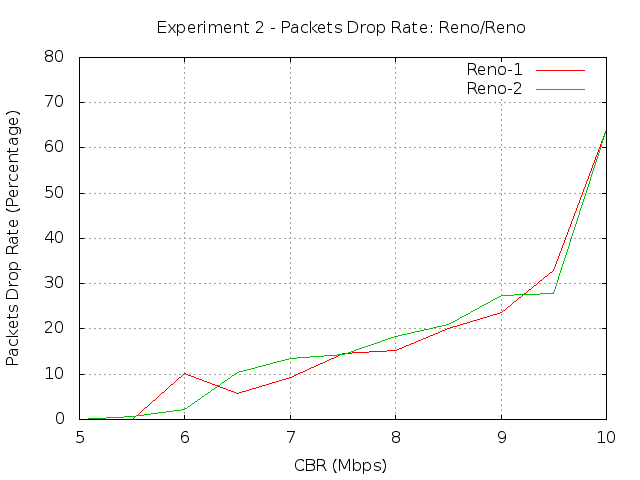
\includegraphics[width=1.0\linewidth]{plot/exp2-dr-Reno-Reno.png}
    \caption{Fairness of Packets Drop Rate on Reno/Reno}
    \label{fig:exp2_dr_rr}
\end{figure}
\begin{figure}[H]
    \centering
    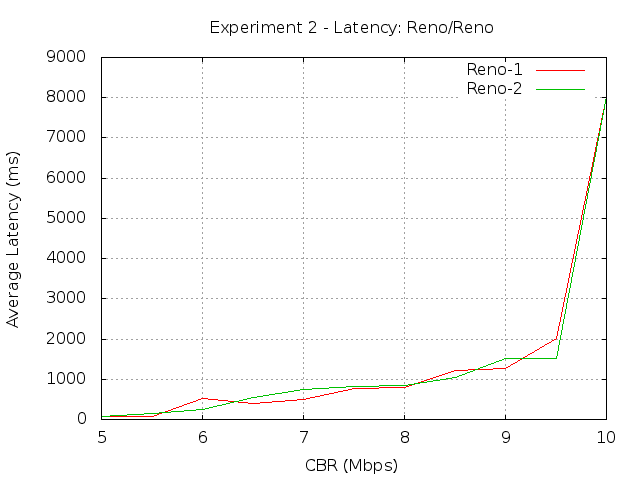
\includegraphics[width=1.0\linewidth]{plot/exp2-lt-Reno-Reno.png}
    \caption{Fairness of Latency on Reno/Reno}
    \label{fig:exp2_lt_rr}
\end{figure}
The result is very clear. As the CBR rate increases, both Reno change 
at the same trend. In all three factors, no single Reno stands out and 
``steals'' all resources. Though there are certain oscillations, it 
still acceptable to say that Reno is fair to another Reno. At a 
congestion network, both Reno are competing for the remaining resource
and alternately occupy more bandwidth for a small amount of time. 

Similar results show in Vegas/Vegas. Figure ~\ref{fig:exp2_thp_vv} shows the Throughput.
\begin{figure}[H]
    \centering
    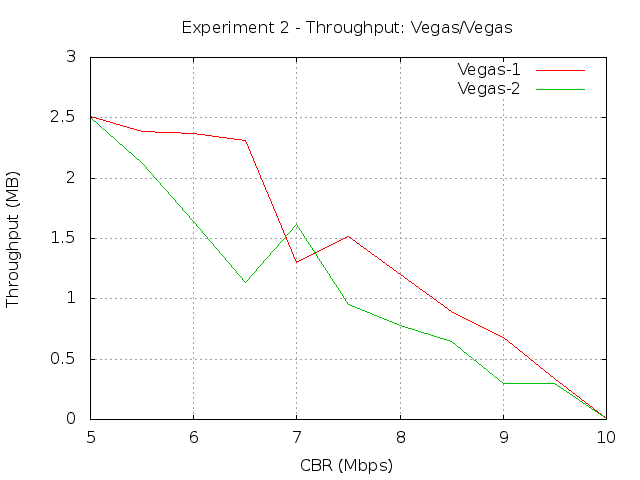
\includegraphics[width=1.0\linewidth]{plot/exp2-thp-Vegas-Vegas.png}
    \caption{Fairness of Throughput on Vegas/Vegas}
    \label{fig:exp2_thp_vv}
\end{figure}
According to this, Reno and Vegas are fair to themselves in most conditions.

\subsection{NewReno/Vegas}
In this simulation, we want to study the fairness between NewReno/Vegas.
Figure ~\ref{fig:exp2_thp_nv}, figure~\ref{fig:exp2_dr_nv} and 
figure~\ref{fig:exp2_dr_nv} shows the Throughput, Packet Drop Rate and 
Latency, respectively.
\begin{figure}[H]
    \centering
    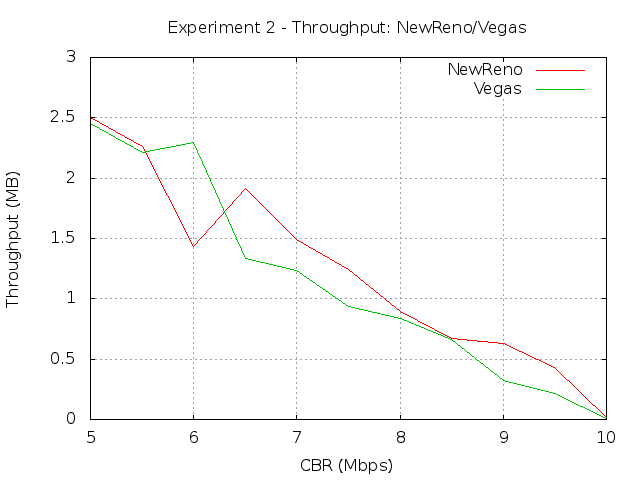
\includegraphics[width=1.0\linewidth]{plot/exp2-thp-NewReno-Vegas.png}
    \caption{Fairness of Throughput on NewReno/Vegas}
    \label{fig:exp2_thp_nv}
\end{figure}
\begin{figure}[H]
    \centering
    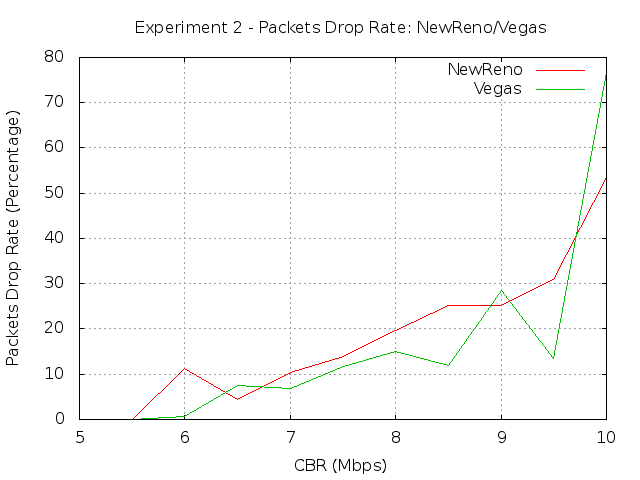
\includegraphics[width=1.0\linewidth]{plot/exp2-dr-NewReno-Vegas.png}
    \caption{Fairness of Packets Drop Rate on NewReno/Vegas}
    \label{fig:exp2_dr_nv}
\end{figure}
\begin{figure}[H]
    \centering
    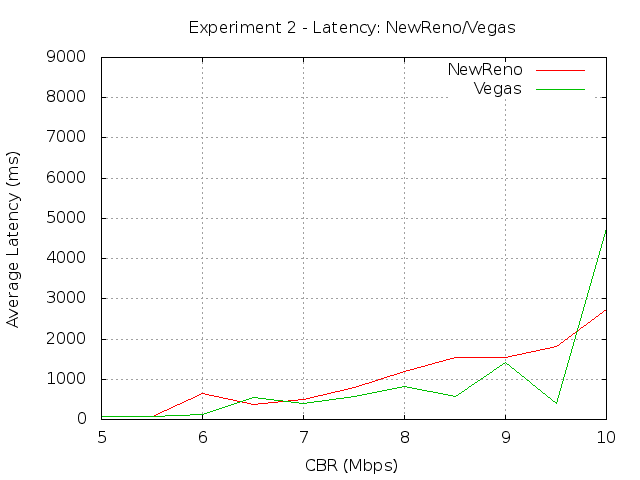
\includegraphics[width=1.0\linewidth]{plot/exp2-lt-NewReno-Vegas.png}
    \caption{Fairness of Latency on NewReno/Vegas}
    \label{fig:exp2_lt_nv}
\end{figure}
As shown, the result is different from last simulation. NewReno
 performs better as CBR rate increases, which means the network is 
 congested and competance is needed for the limited resource. Besides 
 that, NewReno is more steady than Vegas, which means that NewReno is 
 more aggressive and is able to control its own resource, while Vegas
 has to depend on other variants. This is mainly because Vegas uses an
 early congestion detection. Vegas detects congestion early and slows 
 itself down immediately, which in turn gives more bandwidth to NewReno.
 Based on this, I think all other three TCP variants are not fair to Vegas.

\subsection{NewReno/Reno}
In this simulation, we want to study the fairness between NewReno/Vegas.
Figure ~\ref{fig:exp2_thp_nr} and figure~\ref{fig:exp2_dr_nr} shows the Throughput and Packet Drop Rate, respectively.
\begin{figure}[H]
    \centering
    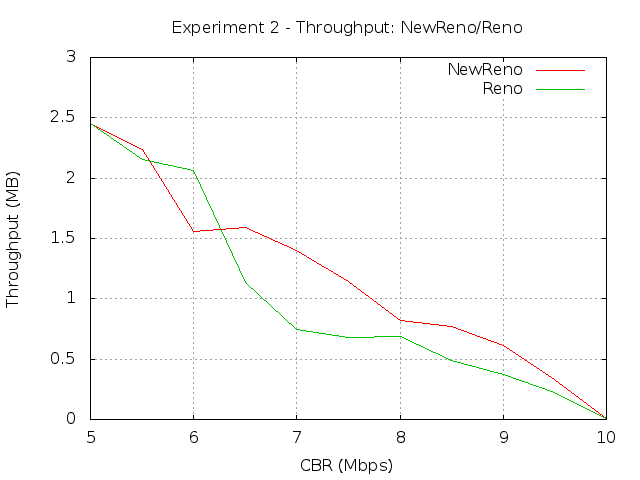
\includegraphics[width=1.0\linewidth]{plot/exp2-thp-NewReno-Reno.png}
    \caption{Fairness of Throughput on NewReno/Reno}
    \label{fig:exp2_thp_nr}
\end{figure}
\begin{figure}[H]
    \centering
    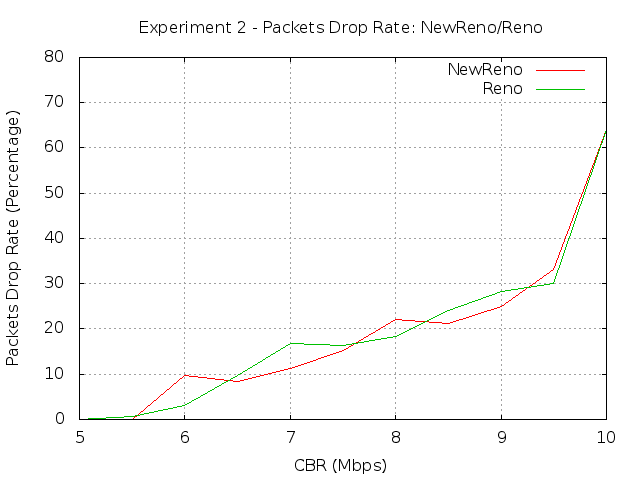
\includegraphics[width=1.0\linewidth]{plot/exp2-dr-NewReno-Reno.png}
    \caption{Fairness of Packets Drop Rate on NewReno/Reno}
    \label{fig:exp2_dr_nr}
\end{figure}
When CBR rate is greater than 7Mbps, NewReno always performs better 
Reno on average throughput. While for the other two factors, latency 
packet drop rate, they are pretty fair to each other. The reason for
this is NewReno improves its retransmission policy agains Reno, and 
is more eager to send more packets, even under a faily small congestion.

For experiment2, we can conclude that each TCP variant is fair to itself. This is because they use the same implementation, and have 
similar anticipates for the same congestion. While for different TCP 
variant pairs, it is unlikely to be fair against each other. This is mainly because they have different reactions to congestion. The early
congestion detection makes Vegas the ``weakest'' because it always 
finds congestion earlier than others, hence slowing down earlier, 
which in turn make others believe the network is better now and 
increase sending rate. For NewReno, once a possible congestion 
detected, more data will be sent to check if it is a real serious 
congestion. 

\section{Experiment 3: Influence of Queuing}
Queuing disciplines like DropTail and Random Early Drop (RED) are 
algorithms that control how packets in a queue are treated. In these 
experiments, instead of varying the rate of the CBR flow, we will 
study the influence of the queuing discipline used by nodes on the 
overall throughput of flows.

The same topology from experiment 1 is used and it has one TCP flow 
(N1-N4) and one CBR/UDP (N5-N6) flow as figure~\ref{fig:exp3_tpg} shows.
\begin{figure}[!htb]
    \centering
    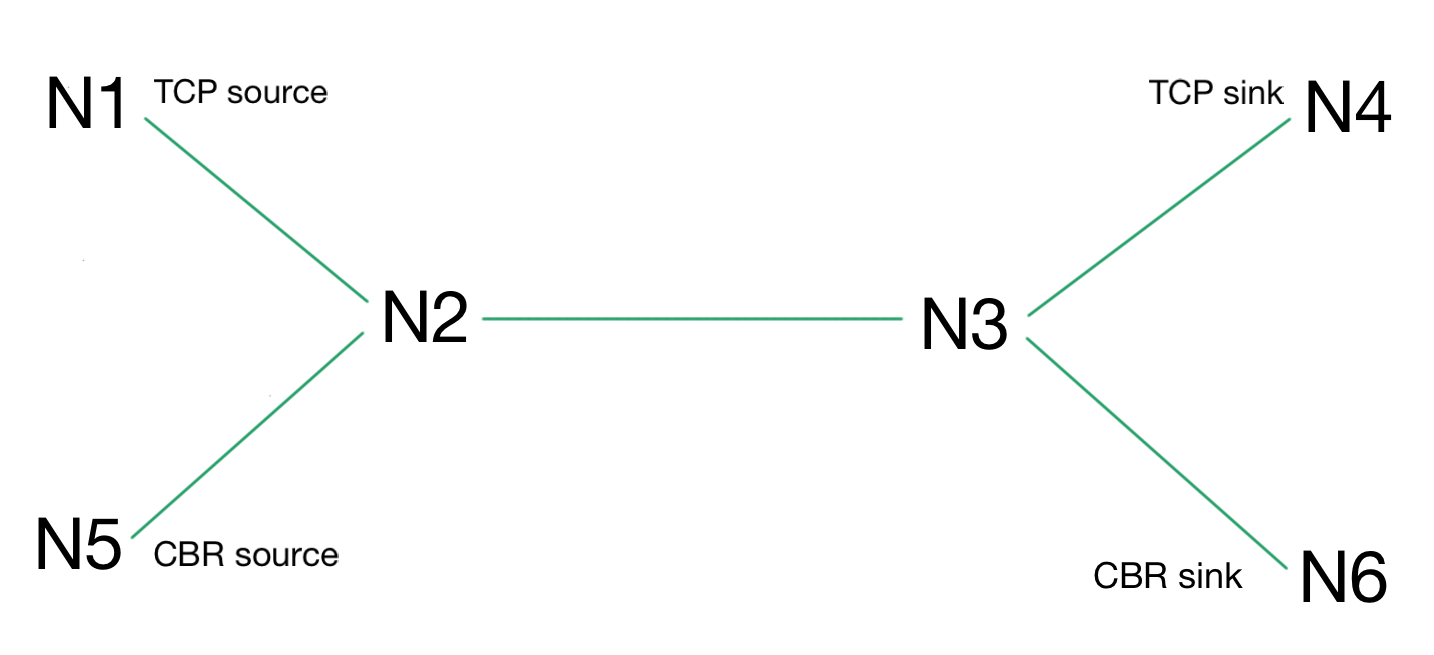
\includegraphics[width=0.8\linewidth]{images/top_exp3.png}
    \caption{Experiment 3 Network Topology}
    \label{fig:exp3_tpg}
\end{figure}
First, TCP flow is started at time 0. Once the TCP flow is steady, the
 CBR source is started, at 15 seconds in our case. CBR flow is stopped 
 at 85 seconds and TCP flow is stopped at 100 seconds. What's TCP 
 window size is 200 and CBR flow rate is 8Mbps.

We are trying to understand how the TCP and CBR flows change under the 
following two different queuing algorithms: DropTail and RED. Also we 
are performing the experiments with two TCP variants Reno and SACK.

\subsection{Average Bandwidth}
The way that we calculate bandwidth over time is by calculating those 
successfully transferred data packets during a short period of time 
$\delta t$. Assume size of each packet is known in advance, total 
number of bytes can be know by multiplying size of packet with number 
of packets that have been transmitted. Then we can know bandwidth B, 
which is  
\begin{center}
    $B = \frac{packetSize \times packetCount}{\delta t}$
\end{center}
For each pair of TCP variant/ queue method, we set the short period of time granularity to be 0.5s, which is described in figure~\ref{fig:exp3-thp}.\\
\begin{figure}[!htb]
    \centering
    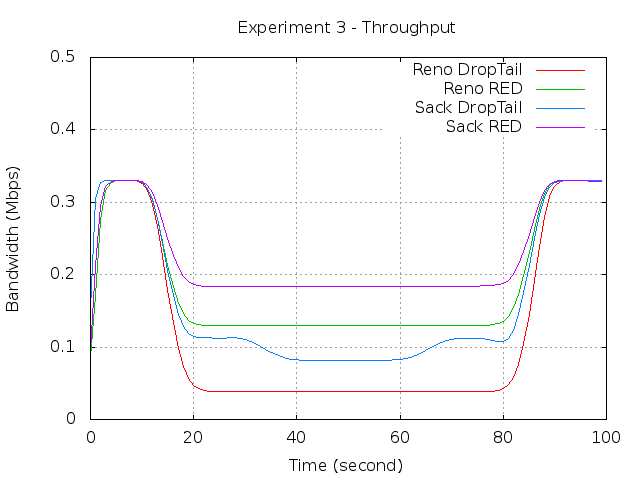
\includegraphics[width=1.0\linewidth]{plot/exp3-thp.png}
    \caption{Average Bandwidth}
    \label{fig:exp3-thp}
\end{figure}
As we can see, before slow start of CBR flow, no what kind of TCP 
variant it is, the TCP flow with DropTail queue method performance 
better than the one with queue method RED. After the slow start of CBR 
flow, although all flows are in state of oscillation, we still can 
conclude that flow with DropTail queue method has a higher throughput 
than RED queue method from the figure. As a result, queuing discipline 
doesn’t provide fair bandwidth to each flow. Overall, DropTail has a 
better performance over RED in regardless of the TCP variant.

During the stage of slow start of CBR flow, different TCP with 
different queue method experience different decrease speed, overall 
Reno with DropTail decrease most sharply. This results from two 
reasons. First, DropTail transmits as many packets as possible unless 
the queue is full. Before CBR flow starts, link between node 1 and 
node 4 has enough brand width for packets to go through. In this case 
very few packets are droped. RED is the policy that drops packets 
randomly even if the queue is not full. Second, during slow start of 
CBR, a lot of packets of the TCP flow are dropped. Reno is going to 
halve the congestion window and set the slow start threshold to new 
congestion window, perform a fast retransmit, and enter a phase called 
Fast Recovery. While SACK retains the slow start part of Reno, it also 
has the coarse grained timeout to fall back on.


After CBR flow gets stable, all TCP flow throughputs decrease to 
stable value comparing to the throughput without CBR flow. Reno with 
queue method RED still has the worst performance, which results from 
randomly dropping packets attribute of RED.

\subsection{Average Latency}
Assume total latency of all packets during a short period of time $\delta t$ and total number of received packets over that short period of time is known, we can know the average latency for each packet during that period of time is 
\begin{center}
    $L = α / (total number of received packets)$
\end{center}
On the basis of each short period, we can accumulatively record latency over the experiment time as the figure~\ref{fig:exp3-lt} describes.
\begin{figure}[!htb]
    \centering
    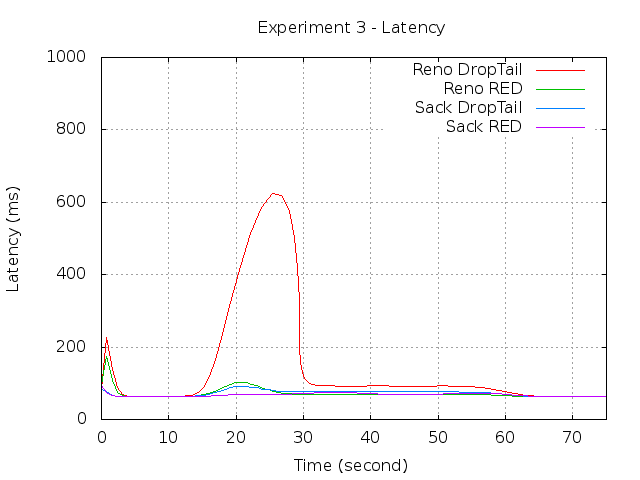
\includegraphics[width=1.0\linewidth]{plot/exp3-lt.png}
    \caption{Average Latency}
    \label{fig:exp3-lt}
\end{figure}
For TCP variant Reno, RED queue method results in a higher latency 
than queue method DropTail overall, which is not surprisingly. The 
most interesting point here is that although SACK with queue method 
RED doesn’t have the best through as shown before, this pair does have 
the remarkable lowest latency no matter with or without CBR flow. This 
shows RED is a good idea while dealing with SACK. At the stage of slow 
start of BCR flow, TCP variant experience a sharp increase of latency 
and RED queue method performs a little better than DropTail as the 
same reasons illustrated before.

Overall, queue method RED has a higher end-to-end latency than 
DropTail, while when RED is combined with TCP variant SACK, it has 
pretty good performance. Reacting to the creation of CBR flow, Reno performs the worst no matter what kind of queue method it is using.


\section{Conclusion}
In this paper, we simulate different TCP variants with NS-2 and analyze the performance of them based on throughput, packets 
drop rate and latency. We also investigate the influence of queuing disciplines to different variants. From the 3 experiments, 
we can conclude that:
\begin{enumerate}
    \item Vegas TCP performs comparatively better than Tahoe, Reno and NewReno TCP.
    \item Same TCP variants are usually fair to each other in the same network. Different variants may have different reaction to possible
    congestion, which may ``steal'' other's resources. 
    \item DropTail has a better performace than RED when considering throughpuy. RED works remarkablely well with SACK TCP, which provides low-latency and more stable transmission.
\end{enumerate}

\end{document}
